
\chapter{Related Work}\label{related}

Clustering is a historically well developed and long lived field in mathematics and computation.  The modern
computational incarnation of clustering likely started with Stuart Lloyd's work in 1957 at Bell Lab's \cite{lloyd-57}.  In the 60 years
since this development, volumes of work have been devoted to developing new methods for identifying clusters and testing
their performance.

Despite an exponential worse-case complexity of $k$-means (where $P\neq NP$) \cite{Vattani}, many real-world problems tend
to fair much better under Lloyd's type of solutions to $k$-means optimization than theoretically optimal solutions.  For
this reason, clustering massive datasets with $k$-means, although suffering from unbounded complexity guarantees, often
yields qualitatively good results close to the optimal $k$-means solution.  Due to the approximate solution's real-world
proclivity towards revealing useful results, randomized methods such as sampling and random dimensional reduction are
often utilized in overcoming complexity growth.  The use of these methods in clustering began with density and grid
based scanning algorithms.

Clustering algorithms have a variety of applicable taxonomies often differentiated by data type, cluster shape,
inference model, and so on.  In this work we will focus mainly on a particular type of clustering distributed algorithms
for clustering high dimensional Gaussian clusters. Below we list some similar clustering methods to RPHash, split by type
and process setting.\\
\noindent
\textbf{Distributed clustering algorithms:}
\begin{itemize}
 \item canopy clustering \cite{mccallum}
\end{itemize}

\noindent
\textbf{Classic algorithms:}
\begin{itemize}
 \item $k$-Means \cite{Hartigan}
 \item $k$-Means++ \cite{arthur-07}
\end{itemize}

\section{Density Based Clustering}

The first set of clustering algorithms began with density based scanning methods.  These methods tend to work well on
spatially separated datasets with relatively low dimension.  A common clustering problem for these types of algorithms
would be on geo-spatial data, in geographic data systems (GIS) and image segmentation.  The algorithms DBScan
\cite{dbscan}, Clique \cite{clique}, and CLARANS \cite{Clarans}, respectively, represent a successful progression of the
density scanning techniques.

%% LEE: streamingRPHash or just RPHash??

DBSCAN proceeds in a conceptually similar manner to \textsf{RPHash} in regard to partitioning the data space
and counting the number of data vectors within a partitioned region.  The first set of parallel clustering algorithms
began with density based scanning methods as the process of building out clusters can take advantage of memory locality
(\emph{e.g.,} spatially near vectors are also near in memory).  Although density scan algorithms are an example of
parallel designed algorithms such as \textsf{RPHash}, they often show weaknesses in accuracy when scaling the number of
dimensions.  A proposed solution mentioned below to this problem is Proclus \cite{Proclus}.

\section{Clustering in Projected Space}

Another important set of algorithms related to \textsf{RPHash} are projection based clustering algorithms.  The natural
commonality among these algorithms is that instead of clustering over the entire data space, they deal with a projected
subset of the data.  The immediate benefit is a reduced computational complexity.  Various other benefits of random
projection are discussed in Section \ref{rpprelim}.  Clustering by random projection, similar to \textsf{RPHash}, are
explored in \cite{fernrandom,alweighted06,avogadri09}, but they often strongly violate the limits of the
\emph{JL}-lemma, resulting in occultation.  The concept of random projection clustering is not new, having been explored
in a variety papers involving high dimensional data clustering.

Proclus \cite{Proclus} was an even early example of projection clustering that used random 1-dimensional projections to
reduce the dimensionality of a clustering problem.  The 1-dimensional projections were then ensembled to create a
consensus of clusters.  A proof of the convergence of projected $k$-means clustering is given in Boutsidis
\cite{Boutsidis}.  The merits of random projection are further discussed in \cite{Dasgupta2000} who suggest that random
projection not only compresses sparse datasets making them computationally more tractable but also may help overall
accuracy by alleviated round-off issues caused by non-homoscedastic variance by generating more spherical clusters in a
more dense subspace.

In addition to Proclus, various other methods and analysis have been proposed for clustering with random projections
that provide bounds on the convergence and limits of random projection clustering.  Florescu gives bounds on the scaling
and convergence of projected clustering \cite{florescu09}. Their results closely follow the logic of Urruty
\cite{Urruty2007}, and find that the number of orthogonal projections required, is logarithmic in $n$, the number of
vectors to be clustered.  Related to the arctangent of the angle between any two distinct clusters the probability of a
random projection plane offering a good partitioning increases exponentially as the number of dimensions in the
projected subspace increases.  Bingham \emph{et al} provide examples of projected clustering well below the JL bound
\cite{bingham} and Bartal \emph{et al} make these assertions mathematically rigorous showing that the projected subspace
is independent of the data's original dimensionality \cite{bartal}.
%FEATURE Selection
Proclus used an assumption similar to \textsf{RPHash} regarding high dimensional data's sparseness.  Feature subset
selection offers a way of compacting the problem as well as removing artifacts.  Many subset selection algorithms have
been explored \cite{subset1,subset2,Yang,Kaski98}.  They generally require difficult to parallelize iterative gradient
descent \cite{Amdahl} or tree traversal \cite{Freeman}.  Random projection is performed on the data to compress it to
spherical clusters \cite{Dasgupta2000} in a dense subspace.  An iterative method for k-medoid search, similar to CLARANS
\cite{Clarans} is then used to identify clusters.  Although the proposed method is successful in accelerating larger
dimensionality problems ($~d=20$) it does not have the overall proposed scalability of \textsf{RPHash}.  This is due to
Proclus being based on an ultimately iterative algorithm, containing inevitably sequential code, and therefore lacking
indefinite scalability \cite{Amdahl}.

Other clustering by random projection algorithms have been explored that are similar to \textsf{RPHash}, but for
projections on the line.  These so called cluster ensemble approaches \cite{fernrandom,alweighted06,avogadri09} use
histograms to identify cluster regions of high density much like \textsf{RPHash}.  Although, as suggested in Florescu and
Urruty, the single dimension approach may be plagued by issues of occultation, and exponential convergence as $d$
increases.  Figure \ref{3dto2d} shows a brief example of projection occultation for Gaussian clusters in $\mathbb{R}^3$
space, projected to $\mathbb{R}^2$ space.  In Figure \ref{3dto2d} it is clear that even modest reductions of $3$
dimensions to $2$ dimensions can yield unwanted results.

\begin{figure}
    \centerline{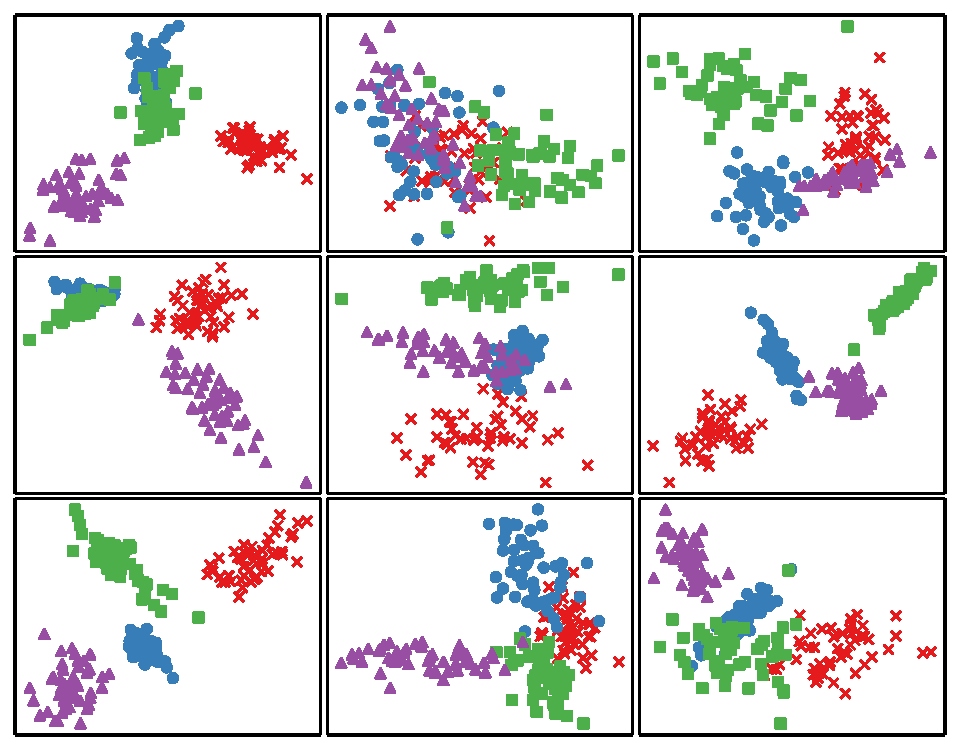
\includegraphics[width=.70\textwidth]{figs/3dto2dproj}}
    \caption{Random Projection of Gaussian Clusters in $\mathbb{R}^3\rightarrow \mathbb{R}^2$}
    \label{3dto2d}
\end{figure}
%%Recently, a streaming version of $k$-means, Streaming $k$-means \cite{stream$k$-means} was 
%%proposed that uses divide and conquer techniques along with sampling to solve the
%%Approximate $k$-means clustering problem.

\section{Streaming Algorithms}

Streaming Clustering is subset of clustering that consists of clustering data that arrives in a streaming fashion or as
batches overtime.  The goal is to perform a similar partitioning as the static case for other clustering methods with
the requirement that we cannot randomly access seen data, nor see future data.  CluStream \cite{clustream} is a
framework for clustering dynamic streaming data.  CluStream stores micro-clusters, consisting of a over sampling of the
$k$ desired clusters.  The $k$ desired partitions are emitted at chosen time intervals, through some off-line clustering
method, thus leading to on-line and off-line clustering phases.  In addition addition, CluStream allows for dynamic
clustering by introducing Pyramidal Time Frames that allow micro-clusters to split and merge over time.  The CluStream
framework is applicable to a variety of streaming clustering methods, and its on-line/off-line phase decomposition is
the general framework adopted by Tree-Walk \textsf{RPHash}.

A common baseline algorithm for streaming clustering, called streaming $k$-Means\cite{braverman,streamkmeans} derives much of its update process from
the original Lloyd-type $k$-Means iteration.  However, similar to CluStream, an over-estimate of micro-clusters is
maintained, to be further clustered in an off-line step.  Streaming $k$-Means' similarity to $k$-Means, is in its process of
assigning incoming vectors to their nearest representative cluster.  However due to the ground state of not having
clusters, the decision whether to aggregate with an existing cluster or form a new one must be made.  In general this
can be done with some sort of inter-cluster similarity or intra-cluster dissimilarity metric.  Some of the drawbacks to
streaming $k$-Means is that it is highly dependent on the input order of the data stream.

%% sliding window
In addition to random projection methods, recently streaming algorithms for data clustering are also considered
\cite{Har-Peled,braverman}.  The general setup of these algorithms consists of a diminishing objective bound that
tightens as the stream is processed.  The processor updates the core-sets of pseudo-centroids when data are within the
objective bound, and disregards data outside that bound.  Streaming $k$-means algorithms perform well on data streams,
but have the drawback of requiring that data be `well-clusterable'.  \textsf{streamingRPHash} uses a similar core-set
approach, but instead of choosing core-sets based on computed distances from current centroids, it maintains a data
structure of dense partitioned regions.

CSketch is a streaming algorithm for generating clusters over massive-domain datasets \cite{aggarwal}.  It shares much
in common with \textsf{streamingRPHash}.  In particular, CSketch applies the Count-Min Sketch data structure to update
candidate centroids by updating the centroid location and not just a count.  Incoming centroids must then search for
candidate clusters in order to find the nearest centroid.  In \textsf{streamingRPHash} we use the LSH decoding of
projected points to immediately find the nearest candidate cluster in the Count-Min Sketch data structure.  Furthermore,
our hashing algorithm is intrinsic to the decoding step, and does not require a supplementary hashing scheme.

\section{Tree Based Clustering}

A later enhancement to \textsf{RPHash} referred to as adaptive LSH (ALSH), and its subsequent alternative tree-walk,
off-line-step shares similarities with the decision tree clustering discussed in ``Clustering Through Decision Tree
Construction'' \cite{Liu2000}.  Liu \emph{et al} describe an implicit clustering approach that instead of grouping
observations by inter-cluster similarity (such as WCSSE), attempts to differentiate dense clusterable data from
uniformly distributed background data.  Like decision trees, the CLTree algorithm recursively splits the data set into
groups of similar observations.  An unsupervised optimization condition is required to overcome the discord between
unsupervised clustering, embedded in a supervised learning algorithm like decision trees.  The condition, mention
previously is to assume points belong to either a dense cluster or are part of some random uniform background noise.  To
differentiate clusters, from noise Liu \emph{et al} optimize the information gain criterion C4.5 at each split.  As such,
CLTree iterates over the dimensions in the data space, splitting the dataset with the hyperplane that maximizes the
information gain criterion for that dimension.  A further modification of the information gain criterion, by which the
algorithm ``looks forward'' a set number of levels of the tree, prevents decision plane from directly cutting clusters
in half.  The method is primarily concerned with lower dimensional clustering tasks for less than 20 dimensions, and has
roughly linear complexity over dimensionality and dataset sizes up to 20 dimensions and 500000 records respectively.
These results are on par with the results for \textsf{RPHash}.  A caveat with their results is that each cluster was
specifically generated to occupy a completely independent subspaces from the other clusters, and that subspace spans less than
five dimensions.
